\chapter{IPv6 - A first Glance}
\label{IPv6 - A first Glance}

\section{Setting Kathara Configuration files}
\begin{figure}[H]
\centering
  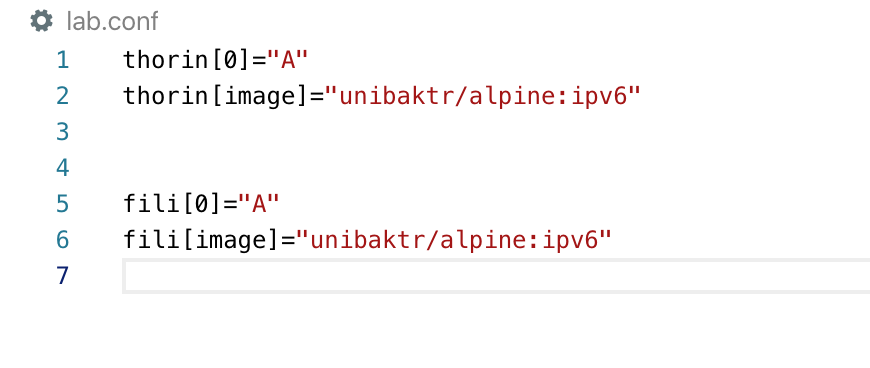
\includegraphics[width=0.9\textwidth]{images/confFile.png}
  \caption{Configuration of labConf file}
  \label{fig: 1.1}
\end{figure}

\subsection{Startup files for Thorin and fili}
\begin{figure}[H]
  \centering
  \begin{minipage}[b]{0.45\textwidth}
    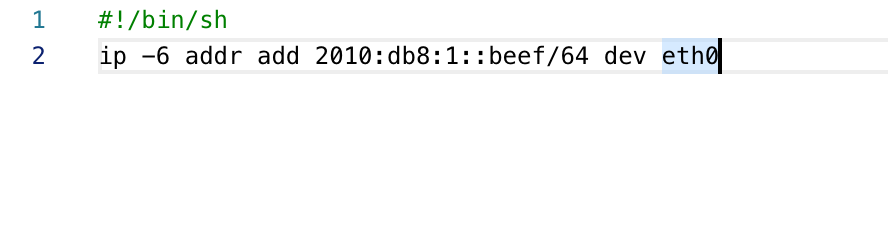
\includegraphics[width=\textwidth]{images/filiStartup.png}
    \caption{Fili startup file.}
  \end{minipage}
  \hfill
  \begin{minipage}[b]{0.45\textwidth}
    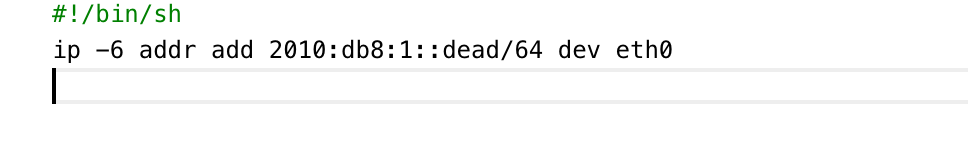
\includegraphics[width=\textwidth]{images/thorinStartup.png}
    \caption{Thorin startup file.}
  \end{minipage}
\end{figure}


\section{Congiguring Kathara settings to in enable IPv6}

\begin{figure}[H]
  \centering
  \begin{minipage}[b]{0.45\textwidth}
    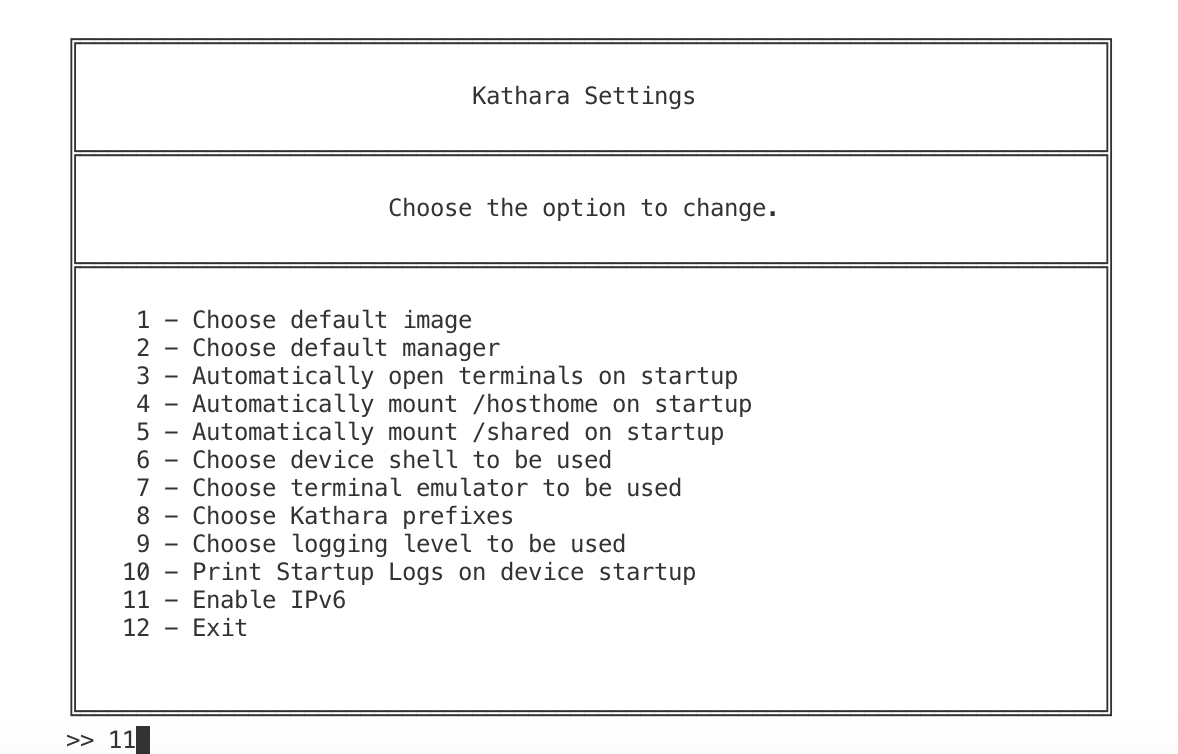
\includegraphics[width=\textwidth]{images/KatharaSettings.png}
    \caption{Enabling IPv6 in Kathara}
  \end{minipage}
  \hfill
  \begin{minipage}[b]{0.45\textwidth}
    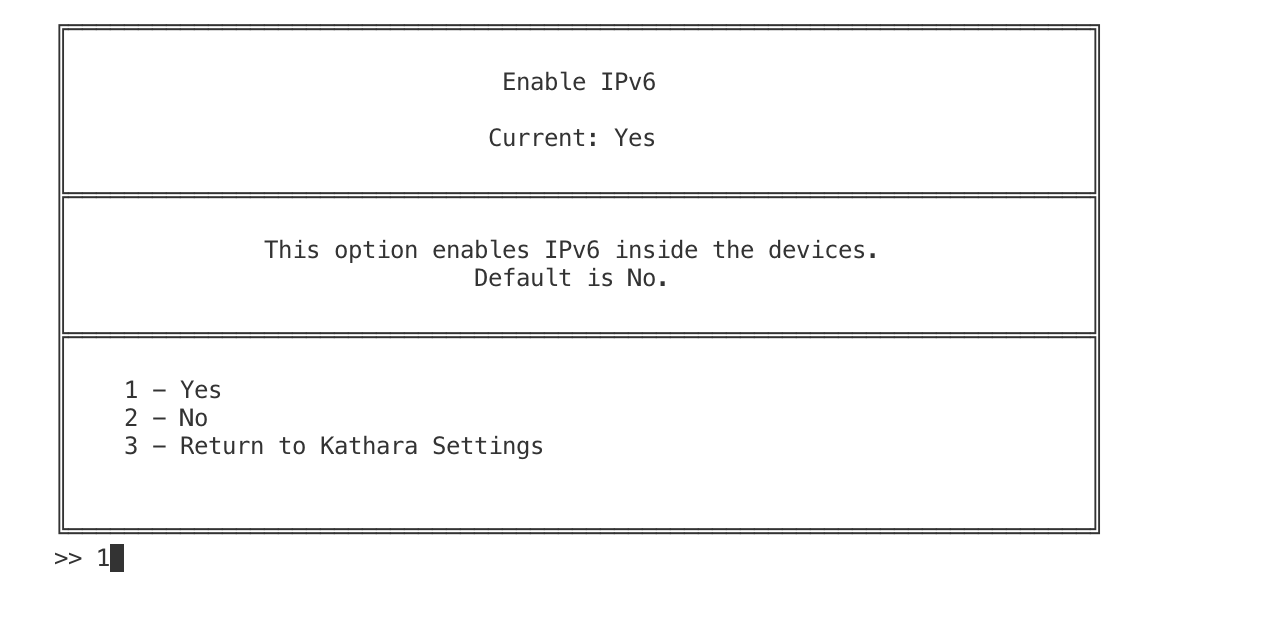
\includegraphics[width=\textwidth]{images/katharaSetiingConfir.png}
    \caption{Saving settings}
  \end{minipage}
\end{figure}

\section{checking connectivity between the hosts}
In this section we check the connectivity between host by using IPV6 commands.
\begin{itemize}
    \item ping6
    \item traceroute6
\end{itemize}

\begin{figure}[H]
\centering
  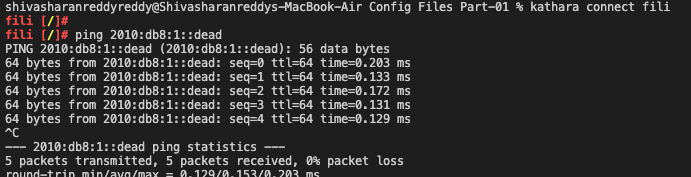
\includegraphics[width=0.9\textwidth]{images/Ping from fili to thorin .png}
  \caption{ping from thorin to fili}
  \label{fig: 1.2}
\end{figure}

\begin{figure}[H]
\centering
  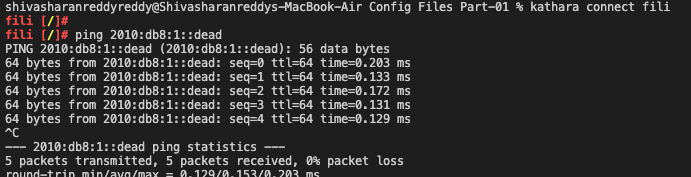
\includegraphics[width=0.9\textwidth]{images/Ping from fili to thorin .png}
  \caption{ping from thorin to fili}
  \label{fig: 1.3}
\end{figure}
\section{Describing features in IPv6 not in IPv4}
IPv6 includes the following features that fix most of the limitations of IPv4
\begin{itemize}
\item \textbf{New Header Format.}
\\ The IPv6 header has a new format designed to minimize header overhead and this optimization is achieved by moving both non-essential fields and optional fields to extension headers that appear after the IPv6 header. IPv4 headers and IPv6 headers do not interoperate. IPv6 is not a superset of functionality that is backward compatible with IPv4.
\\A host or router must use an implementation of both IPv4 and IPv6 to recognize and process both header formats. The IPv6 header is only twice as large as the IPv4 header, even though IPv6 addresses are four times as large as IPv4 addresses.
 \item \textbf{Larger Address Space.}
\\ IPv6 has 128-bit (16-byte) source and destination IP addresses. Although 128 bits can express over 3.4*1038 possible combinations, the large address space of IPv6 has been designed for multiple levels of subnetting and address allocation from the Internet backbone to the individual subnets within an organization. 
\\With a much larger number of available addresses, address-conservation techniques, such as the deployment of NATs, are no longer necessary.
\item \textbf{Efficient and Hierarchical Addressing and Routing Infrastructure.}
\\IPv6 global addresses that are used on the IPv6 portion of the Internet are designed to create an efficient, hierarchical, and summarizable routing infrastructure that is based on the common occurrence of multiple levels of Internet service providers.
\item \textbf{Stateless and Stateful Address Configuration.}
\\ To simplify host configuration, IPv6 supports both stateful address configuration (as in the presence of a DHCP server) and stateless address configuration (as in the absence of a DHCP server).
\\With stateless address configuration, hosts on a link automatically configure themselves with IPv6 addresses for the link (called link-local addresses) and with addresses that they derive from prefixes that local routers advertise. Even in the absence of a router, hosts on the same link can configure themselves with link-local addresses and communicate without manual configuration.
\item \textbf {Built-in Security.}
\\ The IPv6 protocol suite requires support for IPSec. This requirement provides a standards-based solution for network security needs and promotes interoperability between different IPv6 implementations.
\item \textbf{Better Support for QoS.}
\\ New fields in the IPv6 header define how traffic is handled and identified. Traffic identification (using a Flow Label field in the IPv6 header) allows routers to identify and provide special handling for packets belonging to a flow, which is a series of packets between a source and a destination. Because the IPv6 header identifies the traffic, QoS can be supported even when the packet payload is encrypted through IPSec.
\item \textbf {New Protocol for Neighboring Node Interaction.}
\\ The Neighbor Discovery protocol for IPv6 is a series of Internet Control Message Protocol for IPv6 (ICMPv6) messages that manage the interaction of nodes on the same link (known as neighboring nodes). Neighbor Discovery replaces the broadcast-based Address Resolution Protocol (ARP), ICMPv4 Router Discovery, and ICMPv4 Redirect messages with efficient multicast and unicast Neighbor Discovery messages.
\item \textbf {Extensibility.}
\\ IPv6 can easily be extended by adding extension headers after the IPv6 header. Unlike options in the IPv4 header, which can support only 40 bytes of options, the size of IPv6 extension headers is constrained only by the size of the IPv6 packet.
\end{itemize}

\section{Difference between stateful and stateless auto configuration}
The \textbf{stateless} approach is used when user wants to configure a node without concerning a server to maintain any dynamic state for the node. In this case, user can get prefixes and routes from router advertisements and choose its own addresses. However, the address still must be unique and properly routable.
While in  \textbf{stateful} DHCPv6 approach , the server handles configuration, like in IPv4 DHCP. This method is used when a site requires more precise control over address assignments.
\newline{Using \textbf{stateful} DHCP (v4 or v6) a client is more likely to keep a stable IP as long as it is on the same network, while with \textbf{stateless} method it will change frequently.}



